\section{历史信息与自适应更新}
\label{sec:opt-sto-adaptive}

上一节用历史读数纠正方向的偏离。本节研究历史读数的另一种用法：根据过去读数的幅度为各个坐标或各个矩阵方向确定尺度。这些机制同样可以用于精确梯度，第~\ref{chap:opt-smooth}章的动量就是用历史形成方向的例子；与随机读数结合时，尺度本身也成了随机量，原来的偏差与收敛分析需要重新检查。本节只收纳确实维护历史统计的方法。步长调度已在第~\ref{sec:opt-sto-schedules}节随随机梯度建立，裁剪和替代梯度改变的是读数本身，放在第~\ref{sec:opt-sto-direction}节。

\subsection{累计尺度与AdaGrad}
\label{sec:opt-sto-adagrad}

\paragraph{逐坐标的累计尺度}
设想一个文本分类问题，特征是词是否出现。常见词几乎在每个样本中出现，对应坐标的读数每步都不为零；罕见词偶尔出现，对应坐标大多数时候读数为零。用同一个步长，常见词坐标被频繁推动，罕见词坐标几乎不动。AdaGrad为每个坐标记录读数平方的累计和，用它的平方根去除当前读数\scite{duchi2011adagrad}。取$\bm v^{(0)}=\bm0$、步长$\eta>0$与稳定常数$\epsilon>0$，每轮依次执行
\begin{equation}
\label{eq:opt-sto-adagrad}
  \bm v^{(t+1)}=\bm v^{(t)}+\bm g^{(t)}\odot\bm g^{(t)},\qquad
  \bm x^{(t+1)}=\bm x^{(t)}-\eta\,\frac{\bm g^{(t)}}{\sqrt{\bm v^{(t+1)}}+\epsilon},
\end{equation}
其中$\odot$、平方根和除法都逐坐标进行。顺序是先读数、再用本轮读数更新统计、最后用新统计缩放本轮读数。稳定常数放在根号外，只为避免分母为零；有的实现把它放在根号内，两者在$\bm v$很小时行为不同，须按实际实现记录。

这里的尺度来自读数的历史二阶矩，一般不是目标的Hessian。对一维二次函数$f(x)=\tfrac h2x^2$，精确梯度为$hx$，累计量是$\sum_sh^2(x^{(s)})^2$，它同时取决于曲率$h$和走过的路径，并不等于$h$。逐坐标除以历史幅度，可以看作一种随时间变化的对角缩放，但它不是对固定曲率的近似。

\paragraph{两个坐标的短序列}
取$\eta=1$、忽略$\epsilon$。坐标$1$每轮读数都是$1$，坐标$2$只在$t=0$与$t=4$读数为$1$，其余时刻为零。表~\ref{tab:opt-sto-adagrad-steps}列出各轮实际作用在非零读数上的系数$\eta/\sqrt{v_k^{(t+1)}}$。坐标$1$的系数按$1/\sqrt{t+1}$持续缩小，到第$4$轮是$0.447$；坐标$2$的累计量只在它真正出现时增长，第$4$轮的系数仍有$0.707$。稀疏坐标因此保留了较大的有效步长。表中右侧是下一小节的RMSProp（$\rho=0.9$），供比较。

\begin{table}[!htbp]
  \centering
  \small
  \caption{两个坐标上AdaGrad与RMSProp的有效系数$\eta/\sqrt{v_k^{(t+1)}}$（$\eta=1$，忽略稳定项）。坐标$1$每轮读数为$1$；坐标$2$只在$t=0,4$读数为$1$，其余轮读数为零、不发生位移，记为“—”。}
  \label{tab:opt-sto-adagrad-steps}
  \begin{tabular}{ccccc}
    \toprule
    & \multicolumn{2}{c}{AdaGrad} & \multicolumn{2}{c}{RMSProp}\\
    \cmidrule(lr){2-3}\cmidrule(lr){4-5}
    轮次$t$ & 坐标$1$ & 坐标$2$ & 坐标$1$ & 坐标$2$\\
    \midrule
    $0$ & $1.000$ & $1.000$ & $3.162$ & $3.162$\\
    $1$ & $0.707$ & — & $2.294$ & —\\
    $2$ & $0.577$ & — & $1.921$ & —\\
    $3$ & $0.500$ & — & $1.705$ & —\\
    $4$ & $0.447$ & $0.707$ & $1.563$ & $2.457$\\
    $5$ & $0.408$ & — & $1.461$ & —\\
    \bottomrule
  \end{tabular}
\end{table}

\paragraph{存储与长期缩步}
AdaGrad的额外状态是一个$d$维向量，每轮额外计算$O(d)$。累计量只增不减，因此每个坐标的有效步长单调变小。对读数幅度大致恒定的坐标，有效步长按$1/\sqrt t$衰减，这与凸在线问题的需要相符；但对非凸训练，早期的大读数会永久压低后期步长，算法可能在远未收敛时就几乎停止移动。

\paragraph{保证的范围}
AdaGrad最初的分析针对凸的在线学习：在可行域有界、读数有界等条件下，累计损失与最优固定决策之差按$O(\sqrt T)$增长，且对稀疏读数有更好的常数\scite{duchi2011adagrad}。确定性光滑问题、随机凸问题和非凸问题上的分析各有不同的假设与结论，引用时须注明属于哪一种。仅从更新形式不能推出“对任何问题都比梯度下降快”：逐坐标缩放只有在问题的难点与坐标轴对齐时才有明显收益，图~\ref{fig:opt-sto-adaptive-paths}会给出反例。

\subsection{衰减统计与Adam}
\label{sec:opt-sto-adam}

\paragraph{RMSProp：让旧尺度逐渐遗忘}
AdaGrad的累计量无法忘记早期的大读数。RMSProp把累计和换成\term{指数移动平均}（exponential moving average）\scite{hinton2012rmsprop}：
\[
\begin{aligned}
  \bm v^{(t+1)}&=\rho\bm v^{(t)}+(1-\rho)\bm g^{(t)}\odot\bm g^{(t)},\qquad\rho\in[0,1),\\
  \bm x^{(t+1)}&=\bm x^{(t)}-\eta^{(t)}\frac{\bm g^{(t)}}{\sqrt{\bm v^{(t+1)}}+\epsilon}.
\end{aligned}
\]
展开递推，$\bm v^{(t+1)}=(1-\rho)\sum_{s\leq t}\rho^{t-s}\bm g^{(s)}\odot\bm g^{(s)}$，大约只记住最近$1/(1-\rho)$轮。读数恒为$g$时$\bm v^{(t+1)}=(1-\rho^{t+1})g^2$：零初始化使早期分母偏小，表~\ref{tab:opt-sto-adagrad-steps}中RMSProp的系数从$3.162$开始，逐渐降向稳态值$1$。

\paragraph{Adam：方向平均与零初始化修正}
Adam在RMSProp之外再对读数本身做指数平均，并修正两个平均的零初始化偏差\scite{kingma2015adam}。取$\bm m^{(0)}=\bm v^{(0)}=\bm0$、$\beta_1,\beta_2\in[0,1)$，每轮读取$\bm g^{(t)}$后依次计算
\begin{align*}
  \bm m^{(t+1)}&=\beta_1\bm m^{(t)}+(1-\beta_1)\bm g^{(t)},&
  \bm v^{(t+1)}&=\beta_2\bm v^{(t)}+(1-\beta_2)\bm g^{(t)}\odot\bm g^{(t)},\\
  \hat{\bm m}^{(t+1)}&=\frac{\bm m^{(t+1)}}{1-\beta_1^{t+1}},&
  \hat{\bm v}^{(t+1)}&=\frac{\bm v^{(t+1)}}{1-\beta_2^{t+1}},
\end{align*}
\[
  \bm x^{(t+1)}=\bm x^{(t)}-\eta^{(t)}\frac{\hat{\bm m}^{(t+1)}}{\sqrt{\hat{\bm v}^{(t+1)}}+\epsilon}.
\]
修正因子的来源是：$\bm m^{(t+1)}=(1-\beta_1)\sum_{s\leq t}\beta_1^{t-s}\bm g^{(s)}$的权重之和为$1-\beta_1^{t+1}$，除以它后权重和为$1$。若读数恒为$\bm g$，则$\hat{\bm m}^{(t+1)}=\bm g$、$\hat{\bm v}^{(t+1)}=\bm g\odot\bm g$，更新为$-\eta\bm g/(|\bm g|+\epsilon)$，在忽略$\epsilon$时是逐坐标的符号步。一般读数序列下，$\hat{\bm m}$是近期读数的加权平均，不等于当前梯度。

Adam的完整状态是参数$\bm x$、两个$d$维向量$\bm m,\bm v$与计数$t$，中断后恢复训练必须一并恢复，否则修正因子与统计都会错位。随机读数下，$\hat{\bm m}^{(t+1)}$与分母都依赖本轮读数，方向的条件期望一般不等于任何确定矩阵乘以$\nabla f(\bm x^{(t)})$，第~\ref{sec:opt-sto-sgd}节的无偏分析不能直接套用。

\paragraph{AMSGrad与AdaDelta}
另外两个变体针对不同的机制。Reddi等构造了一个简单的凸在线问题，说明指数平均的分母可能在大读数过后迅速回落，使有效步长忽大忽小，Adam因此不收敛；AMSGrad的修正是让分母只增不减\scite{reddi2018amsgrad}：在$\bm m,\bm v$的递推之外维护
\[
  \bar{\bm v}^{(t+1)}=\max\bigl(\bar{\bm v}^{(t)},\bm v^{(t+1)}\bigr),\qquad
  \bm x^{(t+1)}=\bm x^{(t)}-\eta^{(t)}\frac{\bm m^{(t+1)}}{\sqrt{\bar{\bm v}^{(t+1)}}+\epsilon}.
\]
若$\eta^{(t)}$也不增，各坐标的有效系数就不增，这是一个代数性质，不是目标值单调，也不是对非凸问题的收敛证明；原论文的保证属于凸在线问题，需要有界域与有界读数。AdaDelta关心的是单位：$\bm g/\sqrt{\bm v}$没有参数的量纲，于是它再记录一份位移平方的平均$\bm r$，用$\sqrt{\bm r}$恢复尺度\scite{zeiler2012adadelta}：
\[
  \begin{gathered}
    \bm\Delta^{(t)}=-\frac{\sqrt{\bm r^{(t)}+\epsilon}}{\sqrt{\bm v^{(t+1)}+\epsilon}}\odot\bm g^{(t)},\qquad
    \bm x^{(t+1)}=\bm x^{(t)}+\bm\Delta^{(t)},\\
    \bm r^{(t+1)}=\rho\bm r^{(t)}+(1-\rho)\bm\Delta^{(t)}\odot\bm\Delta^{(t)},
  \end{gathered}
\]
其中$\bm v$按RMSProp更新。分子必须用旧的$\bm r^{(t)}$，否则本步位移被循环定义。

这些方法都可以写成$\bm x^{(t+1)}=\bm x^{(t)}-\eta^{(t)}\bm D^{(t)}\hat{\bm g}^{(t)}$的形式，$\bm D^{(t)}$是随历史变化的对角矩阵。但$\bm D^{(t)}$依赖本轮或近期的随机读数，既不固定，也不一定有统一的上下界，第~\ref{chap:opt-smooth}章关于固定正定预条件的结论不能直接继承。每种变体的保证都必须连同其假设一起引用。把这些更新与独立于目标梯度的参数收缩组合起来，就得到AdamW；它与在目标中加入$\ell_2$正则项的区别，在第~\ref{chap:opt-function-fitting}章讨论正则化时统一解释。

\paragraph{逐坐标缩放的适用边界}
图~\ref{fig:opt-sto-adaptive-paths}用精确梯度在条件数为$25$的二次函数上比较三种方法。主轴与坐标轴对齐时，AdaGrad第一步恰好是符号步$(+1,-1)$，一步消去陡峭坐标，此后逐坐标的尺度正好抵消两个方向的曲率差异，$60$步后目标值约为$10^{-8}$；Adam因动量而绕行，但仍快于梯度下降。把同一个二次函数旋转$45^\circ$后，陡峭方向不再对应任何一个坐标，逐坐标缩放无法分开两个方向，AdaGrad与Adam的目标值都停在$10^{-2}$量级，与梯度下降相当。逐坐标缩放的收益依赖于坐标系，而不是方法本身的普遍优势。

\begin{figure*}[!htbp]
  \centering
  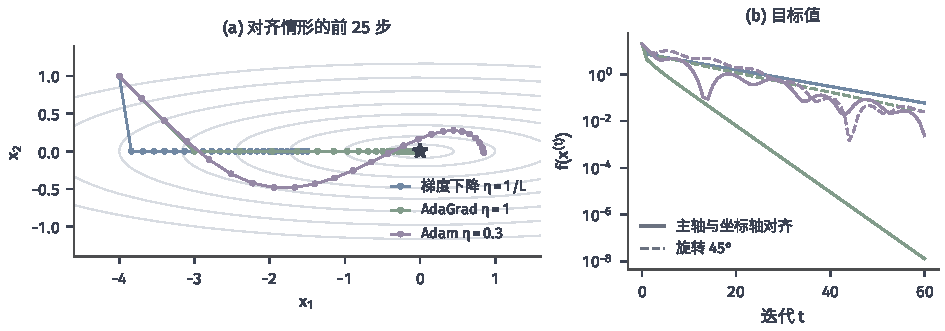
\includegraphics[width=160mm]{figures/03-optimization-evolution-and-signals/01-optimization/matplotlib/c6-adaptive-paths/figure.pdf}
  \caption{逐坐标缩放与坐标系的关系。目标$f(\bm x)=\tfrac12\bm x^\top\bm H\bm x$，精确梯度，初值$(-4,1)$。蓝：梯度下降，步长$1/L=1/25$；绿：AdaGrad，$\eta=1$；紫：Adam，$\eta=0.3$，$\beta_1=0.9$，$\beta_2=0.999$。(a) $\bm H=\operatorname{diag}(1,25)$时前$25$步的路径，灰色为等高线。(b) 目标值：实线为$\bm H=\operatorname{diag}(1,25)$，虚线为把$\bm H$与初值一起旋转$45^\circ$后的同一问题。梯度下降对旋转不变，两条蓝线重合。}
  \label{fig:opt-sto-adaptive-paths}
\end{figure*}

\subsection{Adafactor与统计压缩（补充）}
\label{sec:opt-sto-adafactor}

\paragraph{行列边际代替完整统计表}
神经网络的参数常以矩阵出现。对$\bm W\in\mathbb R^{m\times d}$，Adam式的平方统计$\bm V$与参数同形，要存$md$个数。Adafactor只保存它的行和$\bm R=\bm V\bm 1_d\in\mathbb R^m$与列和$\bm C=\bm V^\top\bm 1_m\in\mathbb R^d$，需要时用
\begin{equation}
\label{eq:opt-sto-adafactor}
  \hat{\bm V}=\frac{\bm R\bm C^\top}{\bm 1_m^\top\bm R}
\end{equation}
重建，存储从$O(md)$降到$O(m+d)$\scite{shazeer2018adafactor}。实际算法对$\bm G\odot\bm G+\epsilon_1$的行列和分别作指数平均，$\epsilon_1>0$保证重建的分母为正；然后用$\bm G/\sqrt{\hat{\bm V}}$作方向，并对这个方向按均方根裁剪、乘以与参数尺度成比例的相对步长。

\paragraph{压缩保留了什么}
式~\eqref{eq:opt-sto-adafactor}的重建保持行和与列和：$\hat{\bm V}\bm 1=\bm R\,(\bm C^\top\bm 1)/(\bm 1^\top\bm R)=\bm R$，列和同理。它丢失的是行列之间的交互。若$\bm V$的元素全为正，则$\hat{\bm V}=\bm V$当且仅当$\bm V$秩为一：若$\bm V=\bm u\bm w^\top$，则$\bm R=\bm u\,(\bm 1^\top\bm w)$、$\bm C=\bm w\,(\bm 1^\top\bm u)$，代入即得$\bm u\bm w^\top$；反之$\hat{\bm V}$按构造是秩一矩阵。例如$\bm V=\begin{bmatrix}1&2\\3&6\end{bmatrix}$可以精确恢复，而$\bm V=\begin{bmatrix}4&1\\1&4\end{bmatrix}$的行和、列和都是$(5,5)$，重建为全部元素等于$2.5$的矩阵，对角线上的大值与非对角的小值被抹平。图~\ref{fig:opt-sto-adafactor}在一个$6\times8$的例子上展示了这种误差：大尺度的行列结构被保留，个别元素的相对误差可达约$0.6$。

\begin{figure*}[!htbp]
  \centering
  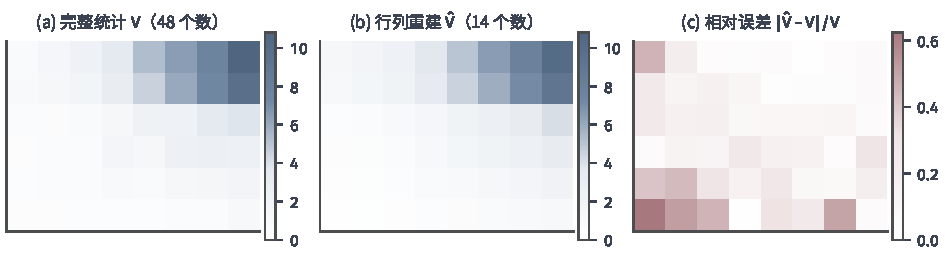
\includegraphics[width=160mm]{figures/03-optimization-evolution-and-signals/01-optimization/matplotlib/c6-adafactor/figure.pdf}
  \caption{平方统计的行列压缩。$40$个随机读数$\bm G_t=(\bm r\odot\bm z_t)\bm c^\top+0.6\bm E_t$，$\bm r$由$2$线性降到$0.5$，$\bm c$由$0.4$线性升到$1.6$，$\bm z_t$与$\bm E_t$为标准正态。(a) 逐元素平方的平均$\bm V$；(b) 由$6$个行和与$8$个列和按式~\eqref{eq:opt-sto-adafactor}重建的$\hat{\bm V}$；(c) 逐元素相对误差，平均约$0.18$，最大约$0.63$。}
  \label{fig:opt-sto-adafactor}
\end{figure*}

近似统计进入实际方向后，方向也随之改变：同一行内各列的相对缩放只由列和决定，无法表达“这一行的第$3$列特别大”。存储的减少与目标下降或收敛速度是两件事，需要分别评价；参数本身、读数和方向的计算仍是$O(md)$，低历史存储也不意味着整次训练的总成本更低。

\subsection{Shampoo与矩阵尺度（补充）}
\label{sec:opt-sto-shampoo}

\paragraph{两侧Gram统计}
逐坐标尺度把矩阵参数的每个元素看成独立的坐标，无法描述“某几行一起变化”这种方向关系。Shampoo为矩阵参数$\bm W\in\mathbb R^{m\times d}$维护左右两个Gram统计\scite{gupta2018shampoo}。取$\epsilon>0$，$\bm L^{(0)}=\epsilon\bm I_m$、$\bm R^{(0)}=\epsilon\bm I_d$，读取同一点的梯度矩阵$\bm G^{(t)}$后先更新统计，再变换方向：
\[
  \begin{gathered}
    \bm L^{(t+1)}=\bm L^{(t)}+\bm G^{(t)}\bm G^{(t)\top},\qquad
    \bm R^{(t+1)}=\bm R^{(t)}+\bm G^{(t)\top}\bm G^{(t)},\\
    \bm W^{(t+1)}=\bm W^{(t)}-\eta\,(\bm L^{(t+1)})^{-1/4}\bm G^{(t)}(\bm R^{(t+1)})^{-1/4}.
  \end{gathered}
\]
两个统计正定，负四分之一次幂由正交谱分解定义：若$\bm L=\bm Q\operatorname{diag}(\lambda_k)\bm Q^\top$，则$\bm L^{-1/4}=\bm Q\operatorname{diag}(\lambda_k^{-1/4})\bm Q^\top$。它们是梯度历史的矩阵函数，而不是目标的Hessian。

只看一步就能理解两侧四分之一次幂的作用。设$\epsilon\to0$，$\bm G$是方阵且可逆，奇异值分解为$\bm G=\bm U\bm\Sigma\bm V^\top$。则$\bm G\bm G^\top=\bm U\bm\Sigma^2\bm U^\top$，$\bm G^\top\bm G=\bm V\bm\Sigma^2\bm V^\top$，
\[
  (\bm G\bm G^\top)^{-1/4}\bm G(\bm G^\top\bm G)^{-1/4}=\bm U\bm\Sigma^{-1/2}\bm\Sigma\bm\Sigma^{-1/2}\bm V^\top=\bm U\bm V^\top ,
\]
所有奇异值被拉平为$1$，只保留奇异方向。例如$\bm G=\operatorname{diag}(4,1/4)$时，两侧的变换都是$\operatorname{diag}(1/2,2)$，方向变为单位矩阵：两个方向的幅度相差$16$倍，变换后相同。累积多步后，统计综合了历史上各方向的幅度，不再是这么干净的形式。

\paragraph{刷新频率与成本}
统计本身的存储为$O(m^2+d^2)$，形成$\bm G\bm G^\top$与$\bm G^\top\bm G$需要$O(m^2d+md^2)$，稠密谱分解求根一次约$O(m^3+d^3)$，应用两侧变换又是$O(m^2d+md^2)$。求根最贵，实际实现常每隔若干步才刷新一次矩阵根，中间沿用旧的根。这样本轮实际使用的尺度来自若干步之前的统计，与公式中的“先更新统计再用新统计”是不同的算法，记录实现时须写明刷新间隔。比较方法时，矩阵存储、分解、刷新和应用的成本都要计入，不能只比较参数更新次数。

\subsection{Lion符号动量法（补充）}
\label{sec:opt-sto-lion}

Lion只保留一个动量向量，并把方向的每个坐标取符号\scite{chen2023lion}。取$\bm m^{(0)}=\bm0$、$\beta_1,\beta_2\in[0,1)$、步长$\eta^{(t)}>0$与参数收缩系数$\lambda\geq0$，每轮依次执行
\[
  \begin{aligned}
    \bm z^{(t)}&=\beta_1\bm m^{(t)}+(1-\beta_1)\bm g^{(t)},\\
    \bm x^{(t+1)}&=\bm x^{(t)}-\eta^{(t)}\bigl(\operatorname{sign}(\bm z^{(t)})+\lambda\bm x^{(t)}\bigr),\\
    \bm m^{(t+1)}&=\beta_2\bm m^{(t)}+(1-\beta_2)\bm g^{(t)},
  \end{aligned}
\]
约定$\operatorname{sign}(0)=0$。构造方向用旧动量$\bm m^{(t)}$与系数$\beta_1$，更新状态用另一个系数$\beta_2$；如果先用$\beta_2$覆盖动量再算方向，就成了另一种算法。

符号运算保留每个坐标的方向，舍弃所有幅度。图~\ref{fig:opt-sto-lion-muon}(a)中，取$\bm m=\bm0$，读数$\bm g_{\mathrm a}=(0.2,0.05)$与$\bm g_{\mathrm b}=(4,1)$方向相同、长度相差$20$倍，Lion给出完全相同的方向$-(1,1)$；方向相近的$\bm g_{\mathrm c}=(3,-0.4)$却因第二坐标符号不同而给出$-(1,-1)$。不计收缩时，若方向有$q$个非零坐标，位移的欧氏范数恰为$\eta^{(t)}\sqrt q$，与读数大小无关。所以Lion的步长与梯度下降或Adam的步长数值不可比，它也不是对原目标的标准梯度步：即使读数是精确梯度，$\operatorname{sign}(\nabla f)$在最小点附近也不会变小，常数步长下迭代会在最小点附近以$\eta$的尺度来回跳动。是否在原目标上取得进展，仍要单独核验目标值或梯度残差。

\subsection{Muon矩阵动量法（补充）}
\label{sec:opt-sto-muon}

\paragraph{用极因子整形动量}
Muon同样处理矩阵参数，但不维护跨步的Gram统计，而是对当步的动量矩阵整形\scite{jordan2024muon}。动量取$\bm M^{(t+1)}=\beta\bm M^{(t)}+\bm G^{(t)}$（Nesterov形式改用$\bm G^{(t)}+\beta\bm M^{(t+1)}$作为待整形的矩阵）。设待整形矩阵$\bm H$的紧奇异值分解为$\bm H=\bm U_r\bm\Sigma_r\bm V_r^\top$，理想的整形输出是\term{极分解}（polar decomposition）中的因子$\bm O=\bm U_r\bm V_r^\top$：保留奇异方向，把所有正奇异值变为$1$。上一小节看到，单步的Shampoo变换给出同一个结果；Muon不累积历史，直接对当步动量求这个因子。

\paragraph{有限次矩阵迭代}
精确的奇异值分解太贵，Muon用矩阵多项式迭代近似极因子。先归一化$\bm X_0=\bm H/\lVert\bm H\rVert_F$，使所有奇异值落在$(0,1]$；再取$(a,b,c)=(3.4445,-4.7750,2.0315)$，执行$5$次
\[
  \bm A_k=\bm X_k\bm X_k^\top,\qquad\bm X_{k+1}=a\bm X_k+(b\bm A_k+c\bm A_k^2)\bm X_k .
\]
每次迭代保持奇异向量不变，把每个奇异值$s$映成$as+bs^3+cs^5$。最后取$\bm W^{(t+1)}=\bm W^{(t)}-\eta\,\gamma_{m,d}\bm X_5$，$\gamma_{m,d}$是依矩阵形状设定的尺度因子，原实现取$\sqrt{\max(1,m/d)}$。图~\ref{fig:opt-sto-lion-muon}(b)画出复合$5$次后的奇异值映射：对$s\in[0.02,1]$，输出落在约$[0.68,1.13]$内来回摆动，而不是精确的$1$。这组系数为了让小奇异值尽快抬升而牺牲了精度；作为对照，经典的三次Newton--Schulz迭代$\bm X_{k+1}=\tfrac32\bm X_k-\tfrac12\bm X_k\bm X_k^\top\bm X_k$在$s\in(0,1)$上单调逼近$1$，但$5$次后$s=0.01$只被抬到约$0.076$。

\begin{figure*}[!htbp]
  \centering
  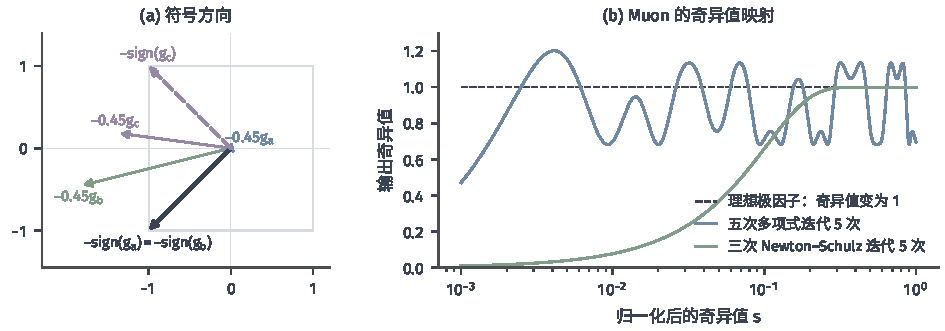
\includegraphics[width=160mm]{figures/03-optimization-evolution-and-signals/01-optimization/matplotlib/c6-lion-muon/figure.pdf}
  \caption{符号方向与奇异值整形。(a) Lion在$\bm m=\bm0$时的方向：细箭头为读数的相反方向$-0.45\bm g$，$\bm g_{\mathrm a}=(0.2,0.05)$、$\bm g_{\mathrm b}=(4,1)$、$\bm g_{\mathrm c}=(3,-0.4)$；粗箭头为$-\operatorname{sign}(\bm g)$，前两者相同，第三个不同。(b) 归一化奇异值$s$经$5$次迭代后的值，横轴为对数坐标：黑色虚线为理想极因子，蓝线为Muon的五次多项式$(a,b,c)=(3.4445,-4.7750,2.0315)$，绿线为三次Newton--Schulz迭代。}
  \label{fig:opt-sto-lion-muon}
\end{figure*}

\paragraph{近似、稳定处理与成本}
因此，实际算法的定义必须包括归一化方式、多项式系数、迭代次数、计算精度以及尺度因子；理想极因子的性质不能直接当作实际输出的性质。$\bm H$的某些奇异值极小时，归一化后的$s$可能低于多项式能有效抬升的范围，对应方向几乎不被放大。每次迭代需要三次矩阵乘法，代价约$O(md\min(m,d))$，$5$次迭代要计入每轮成本。矩阵方向的整形只用到当步动量，不涉及目标的二阶曲率。把参数更新与模型输出分布的几何联系起来的自然梯度、Fisher信息与K-FAC，属于分布几何的内容，可参考\BookChapterRef{chap:information-theory-and-statistical-geometry}{卷四“概率分布的分析与优化”章}。
